\newpage
\section{Aufgabe 1}
\label{sec:a1}

\subsection{a)}
\label{subsec:a1a}
Für den Fluss der Neutrinos ist die Formel
\\
\begin{equation}
  \label{eqn:fluss}
  \Phi = \Phi_{0} \cdot \left( \frac{E}{\si{\tera\electronvolt}} \right)^{-\gamma}
\end{equation}
gegeben. Dabei gilt
\\
\begin{align*}
  \gamma = 2,7
\end{align*}
und für die Energiegrenzen
\\
\begin{align*}
  E_\text{max} &= \infty\\
  E_\text{min} &= \SI{1}{\tera\electronvolt}.
\end{align*}

Im Folgenden wird mit dem Transformationsverfahren eine Funktion erzeugt, die Messergebnisse
für diesen physikalischen Zusammenhang simuliert.
Zuerst wird die Fläche $A$ unter der gesamten Kurve der Funktion \eqref{eqn:fluss} bestimmt:
\\
\begin{align}
  A &= \int_{\SI{1}{\tera\electronvolt}}^{\infty} \Phi_{0}
  \cdot \left( \frac{E}{\si{\tera\electronvolt}} \right)^{-\gamma} \mathrm{d}E\\
  &= - \frac{\Phi_{0}}{\gamma - 1} \cdot \left( 0 - 1 \right)\\
  &= \frac{\Phi_{0}}{\gamma - 1}
\end{align}

Die Fläche unterhalb der Kurve bis hin zur Variablen $E$ ist gegeben durch
\\
\begin{align}
  A(E) &= \int_{\SI{1}{\tera\electronvolt}}^{E} \Phi_{0} \cdot \left( \frac{E}{\si{\tera\electronvolt}}
  \right)^{-\gamma} \mathrm{d}E\\
  &= \frac{\Phi_{0}}{\gamma - 1} \cdot \left( 1 - \left(\frac{E}{\si{\tera\electronvolt}}
  \right)^{-(\gamma -1)} \right)
\end{align}

Es ergibt sich also für die normierte Relativfläche
\\
\begin{equation}
  \label{eqn:relat}
  r(E) = \frac{A(E)}{A} = 1 - \left(\frac{E}{\si{\tera\electronvolt}}\right)^{-(\gamma - 1)}
\end{equation}
Durch Umstellen nach $E$ ergibt sich
\\
\begin{equation}
  \label{eqn:r}
  E(r) = \left( \frac{1}{1 - r} \right)^{\frac{1}{\gamma - 1}}
\end{equation}

\subsection{b)}
\label{subsec:a1b}
Um die Detektionswahrscheinlichkeit zu berücksichtigen, werden $10^{5}$ Zufallszahlen zwischen $0$ und $1$ erzeugt, nun werden die in
\ref{subsec:a1a} simulierten Energiemesswerte in die Formel für die Detektionswahrscheinlichkeit
\\
\begin{equation}
  \label{eqn:detect}
  P(E) = \left( 1 - e^{\frac{-E}{2}} \right)^{3}
\end{equation}
eingesetzt.
Nun wird im Prinzip jedem simulierten Energiewert eine Zufallszahl zugeordnet. Nun weden gemäß dem Neumannschen Rückweisungsverfahren,
alle Zufallszahlen abgelehnt die oberhalb der Detektionswahrscheinlichkeit $P(E)$ liegen. Die jewils zugeordneten Energiewerte werden ebenfalls
abgelehnt, sodass die Energien, jeweils mit der entsprechenden Wahrscheinlichkeit nicht detektiert werden.
Die Ergebnisse von Aufgabe \textbf{a)} und \textbf{b)} sind in Abbildung \ref{fig:plotAB} dargestellt.

\FloatBarrier
\begin{figure}
  \centering
  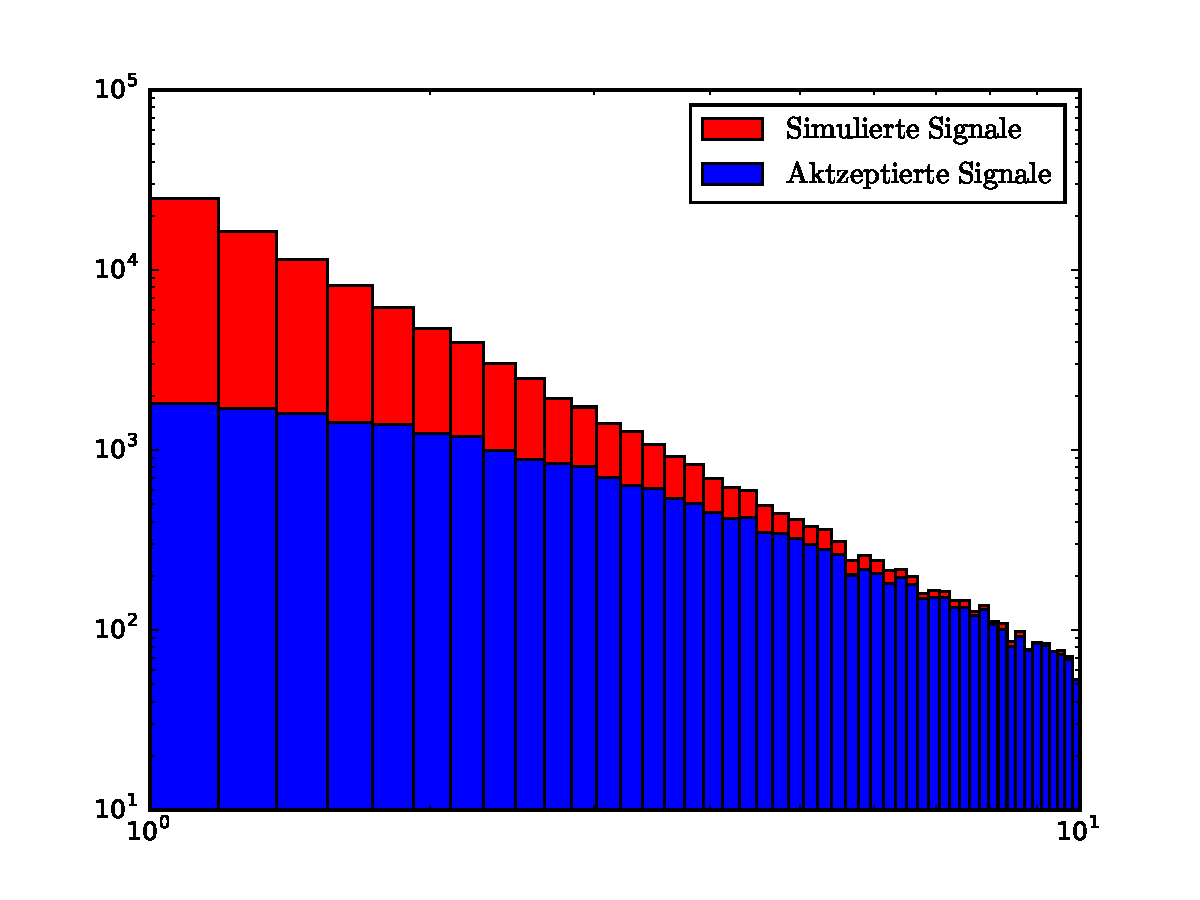
\includegraphics[width=\textwidth]{plotsAB.pdf}
  \caption{Graphische Darstellung der Ergebnisse aus a) und b).}
  \label{fig:plotAB}
\end{figure}
\FloatBarrier


\subsection{c)}
\label{subsec:a1c}
siehe .py Datei.



\subsection{d)}
\label{subsec:a1d}
